\input{../../style/preamble}
\input{../../latex-math/basic-math.tex}
\input{../../latex-math/basic-ml.tex}

\tikzstyle{squ}=[draw, rectangle, minimum size = 5mm]
\tikzstyle{del}=[squ, fill = white]

%\newcommand{\titlefigure}{figure/word_emb.png}
\newcommand{\learninggoals}{
\item Understand the convolution operation and layer
\item Understand applicatoin of CNNs in image analysis
\item Understand applicatoin of CNNs in NLP}

\title{Advanced NN Architectures}
% \author{}
\institute{\href{https://slds-lmu.github.io/lecture_dl4nlp/}{slds-lmu.github.io/lecture\_dl4nlp}}
\date{}

\begin{document}
\lecturechapter{Convolutional Neural Networks}
\lecture{Deep Learning for NLP}

% ------------------------------------------------------------------------------

\begin{vbframe}{neural network architectures}

\vfill

\begin{itemize}
	\item An architecture is an abstract design for a neural network
	\item Loosely speaking: Which nodes connect to which nodes? Which connections share parameters?
	\item Examples of architectures:
		\begin{itemize}
			\item Fully Connected Neural Networks
			\item Convolutional Neural Networks (CNNs)
			\item Recurrent Neural Networks (RNNs)
			\begin{itemize}
				\item Subclasses: Vanilla RNNs, LSTMs, GRUs, QRNNs, ...
			\end{itemize}
			\item Transformers (self-attention)
			\item ...
		\end{itemize}
	\item The choice of architecture is often informed by assumptions about the data, based on our domain knowledge
\end{itemize}

\vfill

\end{vbframe}

% ------------------------------------------------------------------------------

\begin{vbframe}{Assumption of locality}

\vfill

\begin{itemize}
	\item Computer vision: Pixels that make up a meaningful objects tend to be located in a coherent (``local'') area:
\end{itemize}
\begin{tikzpicture}
\node (corgi) at (0,0) {\includegraphics[width=.4\textwidth]{figure/corgi_}};
\node [right=1cm of corgi] {\includegraphics[width=.4\textwidth]{figure/corgi2_}};
\end{tikzpicture}
\begin{itemize}
	\item Not always true for words in NLP:
	\begin{itemize}
		\item \textit{sie sollen sich heute bei ihm im büro \textbf{vorstellen}}
		\item \textit{\textbf{stellen} sie sich bitte heute bei ihm im büro \textbf{vor}}
	\end{itemize}
\end{itemize}

\vfill

\end{vbframe}

% ------------------------------------------------------------------------------

\begin{vbframe}{Assumption of translation invariance}

\vfill

\begin{itemize}
	\item The features that make up a meaningful object do not depend on that object's absolute position in the input.
	\item Computer vision: 
\end{itemize}
\begin{tikzpicture}
\node (corgi) at (0,0) {\includegraphics[width=.4\textwidth]{figure/corgi3_}};
\node [right=1cm of corgi] {\includegraphics[width=.4\textwidth]{figure/corgi4_}};
\end{tikzpicture}
\begin{itemize}
	\item NLP:
		\begin{itemize}
			\item \textit{\textbf{[the yellow house]} [rest of sentence]} $\rightarrow$ noun phrase
			\item \textit{[rest of sentence] \textbf{[the yellow house]}} $\rightarrow$ still a noun phrase
		\end{itemize}
\end{itemize}

\vfill

\end{vbframe}

% ------------------------------------------------------------------------------

\begin{vbframe}{Assumption of sequentiality}

\vfill

\begin{itemize}
	\item NLP: Sentences should be processed left-to-right or right-to-left. This one is falling out of fashion, since people are replacing recurrent neural networks with self-attention networks.
\end{itemize}

\vfill

\end{vbframe}

% ------------------------------------------------------------------------------

\begin{vbframe}{Are these assumptions (always) true?}

\vfill

\begin{itemize}
\item Of course not!
\item But they are a good way of thinking about why certain architectures are popular for certain problems.
\item Also, for limiting the search space when deciding on an architecture for a given project.
\end{itemize}

\vfill

\end{vbframe}

% ------------------------------------------------------------------------------

\begin{vbframe}{Convolutional layers}

\vfill

\begin{itemize}
	\item Technique from Computer Vision (esp. object recognition), by LeCun et al., 1998
	\item Adapted for NLP (e.g., Kalchbrenner et al., 2014)
	\item Filter banks with trainable filters
	\item So what is a filter? What is a filter bank?
\end{itemize}

\vfill

\end{vbframe}

% ------------------------------------------------------------------------------

\begin{vbframe}{Example: 7 day rolling average filter}

\vfill

\begin{center}
\includegraphics[width=.9\textwidth]{figure/covid}
\end{center}

{\hfill \footnotesize \url{https://www.nytimes.com/}, December 07, 2020}

\vfill

\end{vbframe}

% ------------------------------------------------------------------------------

\begin{vbframe}{Example: 7 day rolling average filter}

\vfill

\begin{itemize}
	\item Let $\mathbf{x} \in \mathbb{R}^{J}$ be a vector that represents a data series (e.g., number of positive tests per day, over $J$ consecutive days)
	\item Let $\mathbf{f} \in \mathbb{R}^{K}; \mathbf{f} = [\frac{1}{7}, \frac{1}{7}, \frac{1}{7}, \frac{1}{7}, \frac{1}{7}, \frac{1}{7}, \frac{1}{7}]^T$ be our ``7 day rolling average'' filter vector
	\item Filtering $\mathbf{x}$ with $\mathbf{f}$ (written $\mathbf{f} * \mathbf{x}$) yields a new vector $\mathbf{h}$, with:
	$$h_j = \sum_{k=1}^7 f_{k} x_{(j+k-7)} = \frac{1}{7} (x_{j-6} + \ldots + x_{j})$$
	\item (For now, let's not worry about the edge cases where $j+k-7 \leq 0$.)
\end{itemize}

\vfill

\end{vbframe}

% ------------------------------------------------------------------------------

\begin{vbframe}{1-D convolution}

\vfill

\begin{itemize}
	\item Let's say that we want to train a linear regression model to predict some variable of interest from each datapoint.
	\item Since the raw data is noisy, it makes sense to smoothe it with our rolling average filter first:
	$$\hat{y}_j = wh_j + b; \quad h_j = (\mathbf{f} * \mathbf{x})_j$$
	\item But maybe we should weight the datapoints in our 7-day window differently? Maybe we should give a higher weight to datapoints close to the current day $j$?
	\item We can manually engineer a filter that we think is better, for example:
	\item $\mathbf{f}' = [\frac{1}{10}, \frac{1}{10}, \frac{1}{10}, \frac{1}{10}, \frac{1}{5}, \frac{1}{5}, \frac{1}{5}]^T$
	\item Alternative: Let the \textit{model} choose the optimal filter parameters, based on the training data.
	\item How? Gradient descent!
\end{itemize}

\vfill

\end{vbframe}

% ------------------------------------------------------------------------------

\begin{vbframe}{Backpropagation for 1-D convolution}

\vfill

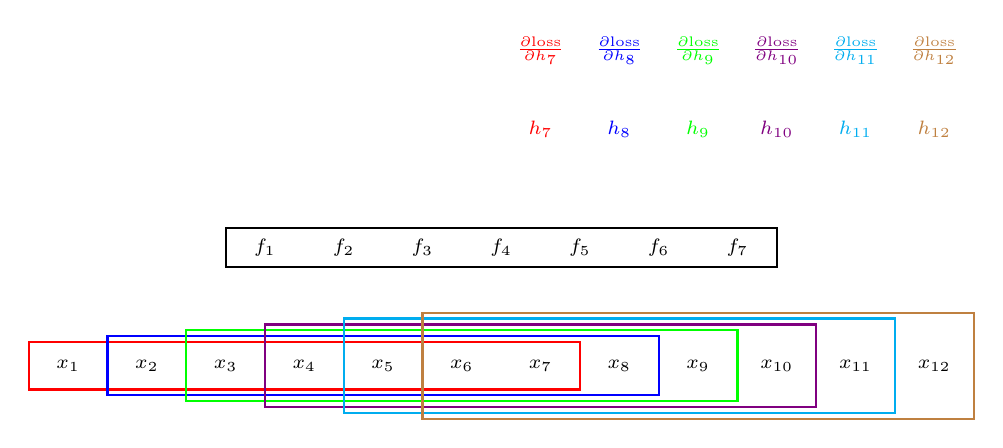
\begin{tikzpicture}
\foreach \i [evaluate=\i as \truei using int(\i+4)] in {-3,...,3}{
\node (f-\i) at (\i+6.5, 1.5) {\scriptsize $f_{\truei}$};
}
\node at (f-0) [draw, thick, rectangle, minimum width=7cm, minimum height=5mm] {};

\foreach \col in {1,...,12}{
\node (n-\col) at (\col, 0) {\scriptsize $x_{\col}$};
}

\foreach \i/\coll [evaluate=\i as \pos using int(\i-3)] in {7/red,8/blue,9/green,10/violet,11/cyan,12/brown}{
\node (y-\i) at (\i, 3) [draw=white, thick, rectangle] {\scriptsize \textcolor{\coll}{$h_{\i}$}};
\node (loss-\i) at (\i, 4) {\scriptsize \textcolor{\coll}{$\frac{\partial \mathrm{loss}}{\partial h_{\i}}$}};
\node at (n-\pos) [draw=\coll, thick, rectangle, minimum width=7cm, minimum height=1.5*\pos mm] {};
}
\end{tikzpicture}

\vfill

\end{vbframe}

% ------------------------------------------------------------------------------

\begin{vbframe}{Convolution as dot products}

\vskip-1mm

\vfill

\begin{tikzpicture}
\foreach \col in {3,...,8}{
\foreach \row [evaluate=\row as \idx using int(\col+\row+1)] in {-3,...,3}{
\node (n-\col-\row) [] at (\col, \row/3) {\scriptsize $x_{\idx}$};}
\node at (n-\col-0) [draw, rectangle, thick, minimum height=2.3cm, minimum width=3.5mm] {};
\foreach \row [evaluate=\row as \truei using int(\row+4)] in {-3,...,3}{
\node (t-\col-\row) [] at (\col, \row/3+3) {\scriptsize $f_{\truei}$};}
\node at (t-\col-0) [draw, thick, rectangle, minimum height=2.3cm, minimum width=3.5mm] {};}
\foreach \row [evaluate=\row as \idx using int(\row-3)] in {-3,...,3}{
\node [left=10mm of n-3-\row] {\scriptsize Shifted by \idx:};
\node [left=3mm of n-3-\row] {$\ldots$};
\node [right=3mm of n-8-\row] {$\ldots$};}
\foreach \col [evaluate=\col as \idx using int(\col+4)] in {3,...,8}{
\node [above = 7mm of t-\col-3, rotate=90, align=center, anchor=center] {\scriptsize $h_{\idx} = \mathbf{f}^T \bar{\mathbf{x}}_{\idx}$};
\node (xbar) [below = 3mm of n-\col--3] {\scriptsize $\bar{\mathbf{x}}_{\idx}$};}
\node (tt) [left=5mm of t-3-0, align=left] {\scriptsize Filter $\mathbf{f}$\\ \scriptsize (same $\mathbf{f}$ for all time steps)};

%\node at (n-3-0) [draw, thick, dashed, rectangle, minimum height=5mm, minimum width=9cm] {};
\end{tikzpicture}

\vfill

\end{vbframe}

% ------------------------------------------------------------------------------

\begin{vbframe}{Backpropagation for 1-D convolution}

\vfill

\begin{itemize}
	\item If we pretend that there is a separate filter parameter $\mathbf{f}_j$ for each $\bar{\mathbf{x}}_j$, then the gradient of the loss w.r.t. that filter would simply be:
	$$\nabla_{\mathbf{f}_j} \mathrm{loss} = \frac{\partial h_j}{\partial \mathbf{f}_j} \frac{\partial \mathrm{loss}}{\partial h_j} = \bar{\mathbf{x}}_j \frac{\partial \mathrm{loss}}{\partial h_j}$$
	\item But of course, there is only one filter. So we add up the gradients for all time steps:
	$$\nabla_\mathbf{f} \mathrm{loss} = \sum_j \nabla_{\mathbf{f}_j} \mathrm{loss} = \sum_j \bar{\mathbf{x}}_j \frac{\partial \mathrm{loss}}{\partial h_j}$$
\end{itemize}

\vfill

\end{vbframe}

% ------------------------------------------------------------------------------

\begin{vbframe}{Bias, nonlinearities, padding, stride (1)}

\vfill

\begin{itemize}
	\item \textbf{Bias and nonlinearities:}
		\begin{itemize}
			\item In a real CNN, we usually add a trainable scalar bias $b$, and we apply a nonlinearity $g$ (such as the rectified linear unit):
			$$h_j = g(b + \sum_{k=1}^K f_k x_{(j+k-K)}) $$
		\end{itemize}
	\item \textbf{Edge cases:}
		\begin{itemize}
			\item Possibel strategies for when the filter overlaps with the edges (beginning/end) of $\mathbf{x}$:
				\begin{itemize}
					\item Outputs where filter overlaps with edge are undefined, i.e., $\mathbf{h}$ has fewer dimensions than $\mathbf{x}$ ($K-1$ fewer, to be exact)
					\item Pad $\mathbf{x}$ with zeros before applying the filter
					\item Pad $\mathbf{x}$ with some other relevant value, such as the overall average, the first/last value, ...
				\end{itemize}
		\end{itemize}
\end{itemize}

\vfill

\end{vbframe}

% ------------------------------------------------------------------------------

\begin{vbframe}{Bias, nonlinearities, padding, stride (2)}

\vfill

\begin{itemize}
	\item \textbf{Stride:}
		\begin{itemize}
			\item The stride of a convolutional layer is the ``step size'' with which the filter is moved over the input
			\item We apply $\mathbf{f}$ to the $j$'th window of $\mathbf{x}$ only if $j$ is divisible by the stride.
			\item In NLP, the stride is usually $1$.
		\end{itemize}
\end{itemize}

\vfill

\end{vbframe}

% ------------------------------------------------------------------------------

\begin{vbframe}{Convolution with more than one axis}

\vfill

\begin{itemize}
	\item Extending the convolution operation to tensors with more than one axis is straightforward.
	\item Let $\mathbf{X} \in \mathbb{R}^{J_1 \times \ldots \times J_L}$ be a tensor that has $L$ axes and let $\mathbf{F} \in \mathbb{R}^{K_1 \times \ldots \times K_L}$ be a filter.
		\begin{itemize}
		\item The dimensionalities of the filter axes are called filter sizes or kernel sizes (``kernel width'', ``kernel height'', etc.)
		\item From now on, we assume that the filter is applied to a symmetric window around position $j$, not just to positions to the left of $j$. (The rolling average was a special scenario, because we assume that future data points $x_{j'}$ with $j' > j$ are not available on day $j$.)
		\end{itemize}
	\item Then the output $\mathbf{H} = \mathbf{F} * \mathbf{X}$ is a tensor with $L$ axes, where:
	$$h_{(j_1, \ldots, j_L)} = g\big(b + \sum_{k_1=1}^{K_1} \ldots \sum_{k_L=1}^{K_L} f_{(k_1, \ldots, k_L)} x_{(j_1 + k_1 - \left\lceil \frac{K_1}{2} \right\rceil, \ldots, j_L + k_L - \left\lceil \frac{K_L}{2} \right\rceil)}\big)$$
\end{itemize} 

\vfill

\end{vbframe}

% ------------------------------------------------------------------------------

\begin{vbframe}{Example: 2D convolution}

\vfill

\begin{tikzpicture}
\foreach \row in {1,...,4}{
\foreach \col/\num [evaluate=\num as \numx using int(\num+\row/2)] in {1/1,2/0,3/1,4/0}{
\node (x-\col-\row) at (\col/2, \row/2) {$\numx$};
}}
\foreach \row/\col in {0/0,0/5,5/5,5/0}{
\node at (\row/2,\col/2) {\textcolor{gray}{$0$}};
}
\foreach \row in {0,5}{
\foreach \col in {1,...,4}{
\node at (\row/2,\col/2) {\textcolor{gray}{$0$}};
\node at (\col/2,\row/2) {\textcolor{gray}{$0$}};
}}

\node [above = 5mm of x-3-4] {Input $\mathbf{X}$ with $J_1=J_2=4$ (padded)\phantom{..}};

\foreach \row in {1,...,3}{
\foreach \col/\num [evaluate=\num as \numx using int(\num+\row/2)] in {1/0,2/1,3/2}{
\node (f-\col-\row) at (\col/2+7, \row/2+4) {$\numx$};
}}
\node at (f-2-2) [rectangle, draw, thick, minimum width=1.5cm, minimum height=1.5cm] {};

\iffalse
\foreach \row [evaluate=\row as \r using int((\row-2)*(-1))]in {1,...,3}{
\foreach \col [evaluate=\col as \c using int(\col-2)] in {1,2,3}{
\node (fx-\col-\row) at (\col*.75+3, \row*.75+3.5) {\tiny $f_{\r, \c}$};
}}
\node at (fx-2-2) [rectangle, draw, thick, minimum width=2.4cm, minimum height=2.5cm] {};
\node [right=5mm of fx-3-2] {$=$};
\fi

\foreach \row in {1,...,4}{
\foreach \col in {1,...,4}{
\node (y-\col-\row) at (\col/2+7, \row/2){};
}}

\node at (y-1-4) {\textcolor{red}{$16$}};
\node at (x-1-4) [rectangle, draw=red, thick, minimum width=1.4cm, minimum height=1.5cm] {};
\node at (y-3-3) {\textcolor{blue}{$26$}};
\node at (x-3-3) [rectangle, draw=blue, thick, minimum width=1.4cm, minimum height=1.5cm] {};
\node at (y-4-1) {\textcolor{green}{$5$}};
\node at (x-4-1) [rectangle, draw=green, thick, minimum width=1.5cm, minimum height=1.5cm] {};

\node at (y-1-3) {$?$};
\node at (y-1-2) {$?$};
\node at (y-1-1) {$?$};

\node at (y-2-4) {$?$};
\node at (y-2-3) {$?$};
\node at (y-2-2) {$?$};
\node at (y-2-1) {$?$};

\node at (y-3-4) {$?$};
\node at (y-3-2) {$?$};
\node at (y-3-1) {$?$};

\node at (y-4-4) {$?$};
\node at (y-4-3) {$?$};
\node at (y-4-2) {$?$};

\node [above = 2mm of y-3-4, align=center] {Output $\mathbf{H}$ with $J_1=J_2=4$ \\ (without bias or nonlinearity)\phantom{..}};
\node [above = 2mm of f-2-3] {Filter $\mathbf{F}$ with $K_2=K_2=3$};

\end{tikzpicture}

\vfill

\end{vbframe}

% ------------------------------------------------------------------------------

\begin{vbframe}{Channels}

\vfill

\begin{itemize}
	\item So far, we have assumed that each position in the input (each day or each pixel) contains a single scalar.
	\item Now, we assume that our input has $M$ features (``channels'') per position, i.e., there is an additional feature axis: $\mathbf{X} \in \mathbb{R}^{J_1 \times \ldots \times J_L \times M}$
	\item Example:
		\begin{itemize}
			\item $M=3$ channels per pixel in an RGB (red/green/blue) image
			\item In NLP: dimensionality of pretrained word embeddings
		\end{itemize}
	\item Then our filter gets an additional feature axis, which has the same dimensionality as the feature axis of $\mathbf{X}$:
	$$\mathbf{F} \in \mathbb{R}^{K_1 \times \ldots \times K_L \times M}$$
	\item During convolution, we simply sum over this new axis as well:
	$$h_{(j_1, \ldots, j_L)} = g\big(b + \sum_{k_1 = 1}^{K_1} \ldots \sum_{k_L = 1}^{K_L}  \sum_{m=1}^M f_{(k_1, \ldots, k_L, m)} x_{(j_1 + k_1 - \left\lceil \frac{K_1}{2} \right\rceil, \ldots, j_L + k_L - \left\lceil \frac{K_L}{2} \right\rceil, m)}\big)$$
\end{itemize}

\vfill

\end{vbframe}

% ------------------------------------------------------------------------------

\begin{vbframe}{Filter banks}

\vfill

\begin{itemize}
	\item A filter bank is a tensor that consists of $N$ filters, which each have the same shape.
	\item The filters of a filter bank are applied to $\mathbf{X}$ independently, and their outputs are stacked (they form a new axis in the output).
	\item So let this be our input and filter bank:
	$$\mathbf{X} \in \mathbb{R}^{J_1 \times \ldots \times J_L \times M}$$
	$$\mathbf{F} \in \mathbb{R}^{K_1 \times \ldots \times K_L \times M \times N}$$
	\item Then our output is a tensor of shape $\mathbf{H} \in \mathbb{R}^{J_1 \times \ldots \times J_L, N}$
		\begin{itemize}
			\item (assuming that we are padding the first $L$ axes of $\mathbf{X}$ to preserve their dimensionality in $\mathbf{H}$)
		\end{itemize}
	\item where $h_{(j_1, \ldots, j_L, n)}$ is same as above
\end{itemize}

\vfill

\end{vbframe}

% ------------------------------------------------------------------------------

\begin{vbframe}{Assumptions behind convolution}

\vfill

\begin{itemize}
	\item Translation invariance: Same object in different positions.
		\begin{itemize}
			\item Parameter sharing: Filters are shared between all positions.
		\end{itemize}
	\item Locality: Meaningful objects form coherent areas
		\begin{itemize}
			\item In a single convolutional layer, information can travel no further than a few positions (depending on filter size)
		\end{itemize}
	\item Hierarchy of features from simple to complex:
		\begin{itemize}
			\item In computer vision, we often apply many convolutional layers one after another
			\item With every layer, the information travels further, and the feature vectors become more complex
			\item Pixels $\rightarrow$ edges $\rightarrow$ shapes $\rightarrow$ small objects $\rightarrow$ bigger objects
		\end{itemize}
\end{itemize}

\vfill

\end{vbframe}

% ------------------------------------------------------------------------------

\begin{vbframe}{Convolution}

\vfill

\begin{center}
\includegraphics[width = 0.4\textwidth]{figure/conv_pool_pic1}
\includegraphics[width = 0.4\textwidth]{figure/conv_pool_pic2}
\end{center}

\footnotesize{Source: Computer science: The learning machines. Nature (2014).}

\vfill

\end{vbframe}

% ------------------------------------------------------------------------------

\begin{vbframe}{Pooling layers (1)}

\vfill

\begin{itemize}
\item Pooling layers are parameter-less
\item Divide axes of $\mathbf{H}$ (excluding the filter/feature axis) into a coarse-grained ``grid''
\item Aggregate each grid cell with some operator, such as the average or maximum
\item Example (shown without a feature axis):
\end{itemize}
\begin{center}
\begin{tikzpicture}

\foreach \i in {0,1,2,3}{
\foreach \j in {0,1,2,3}{
\node [squ] (o\i\j) at (\i*0.5, \j*0.5) {};
} }

\foreach \i in {0,1}{
\foreach \j in {0,1}{
\node [squ] (p\i\j) at (4+\i*0.5,0.5+\j*0.5) {};
} }

\node [above = 5mm of p11.north west] {Max pooled};

\node [] at (o03) {2};
\node [] at (o13) {1};
\node [] at (o02) {1};
\node [] at (o12) {0};
\node [] at (o01) {0};
\node [] at (o11) {4};
\node [] at (o00) {0};
\node [] at (o10) {5};

\node [] at (o23) {2};
\node [] at (o33) {0};
\node [] at (o22) {2};
\node [] at (o32) {0};
\node [] at (o21) {2};
\node [] at (o31) {3};
\node [] at (o20) {1};
\node [] at (o30) {0};

\draw [red, very thick] (o03.north west) -- (o13.north east) -- (o12.south east) -- (o02.south west) -- (o03.north west);

\node [red] at (p01) {2};

\draw [blue, very thick] (o23.north west) -- (o33.north east) -- (o32.south east) -- (o22.south west) -- (o23.north west);

\node [blue] at (p11) {2};

\draw [green, very thick] (o01.north west) -- (o11.north east) -- (o10.south east) -- (o00.south west) -- (o01.north west);

\node [green] at (p00) {5};

\draw [yellow, very thick] (o21.north west) -- (o31.north east) -- (o30.south east) -- (o20.south west) -- (o21.north west);

\node [yellow] at (p10) {3};

\end{tikzpicture}
\end{center}

\vfill

\end{vbframe}

% ------------------------------------------------------------------------------

\begin{vbframe}{Pooling layers (2)}

\vfill

\begin{itemize}
\item When pooling, we lose fine-grained information about exact positions
\item In return, pooling allows us to aggregate features from a local neighborhood into a single feature.
\begin{itemize}
\item For example, if we have a neighborhood where many ``dog features'' were detected (meaning, shapes that look like parts of a dog), we want to aggregate that information into a single ``dog neuron''
\end{itemize}
\end{itemize}

\vfill

\end{vbframe}

% ------------------------------------------------------------------------------

\begin{vbframe}{Convolution and Pooling: LeNet}

\vfill

\begin{itemize}
	\item In computer vision, we often apply pooling between convolutional layers.
	\item Repeated pooling has the effect of reducing tensor sizes.
\end{itemize}
\begin{center}
\includegraphics[width = 0.9	\textwidth]{figure/lenet}
\end{center}
\footnotesize{LeCun et al. (1998). Gradient-based learning applied to document recognition.}

\vfill

\end{vbframe}

% ------------------------------------------------------------------------------

\begin{vbframe}{CNN\lowercase{s} in NLP}

\vfill

\begin{itemize}
	\item Images are 2D, but text is a 1D sequence (of words, n-grams, etc).
	\item Words are usually represented by $M$-dimensional word embeddings (e.g., from Word2Vec)
	\item So on text, we do 1-D convolution with $M$ input features:
		\begin{itemize}
			\item Input matrix: $\mathbf{X} \in \mathbb{R}^{J \times M}$
			\item Filter bank of $N$ filters: $\mathbf{F} \in \mathbb{R}^{K \times M \times N}; K < J$
			\item Output matrix: $\mathbf{H} \in \mathbb{R}^{J \times N}$ 
				\begin{itemize}
					\item (assuming that we padded $\mathbf{X}$ with zeros along its first axis)
				\end{itemize}
		\end{itemize}
	\item Usually, CNNs in NLP are not as deep as CNNs in Computer Vision -- often just one convolutional layer.
\end{itemize}

\vfill

\end{vbframe}

% ------------------------------------------------------------------------------

\begin{vbframe}{Pooling in NLP}

\vfill

\begin{itemize}
\item Pooling is less frequently used in NLP.
\item If the task is a word-level task (i.e., we need one output vector per word), we can simply use the output of the final convolutional layer -- no pooling needed.
\item If the task is some sentence-level task (i.e., we need a single vector to represent the entire sentence), we usually do a ``global'' pooling step over the entire sentence \textit{after} the last convolutional layer:
$$\mathbf{h}_\mathrm{avgpool} = \frac{1}{J} \sum_{j=1}^J \mathbf{h}_j$$

$$\mathbf{h}_\mathrm{maxpool} = \begin{bmatrix} \underset{j}{\mathrm{max}} \quad h_{j,1} \\ \vdots \\ \underset{j}{\mathrm{max}} \quad h_{j,N} \end{bmatrix}$$

\end{itemize}

\vfill

\end{vbframe}

% ------------------------------------------------------------------------------

\begin{vbframe}{CNN\lowercase{s} in NLP}

\begin{center}
\begin{tikzpicture}
\foreach \row in {0,..., 4} {
\foreach \col in {0,..., 7} {
\node (n-\col-\row) at (\col, \row/2) {};
}}

\foreach \col in {0,...,7} {
\node at (n-\col-2) [rectangle, draw, dashed, minimum width=10mm, minimum height=22mm] {};
}
\foreach \row in {0,...,4} {
\node at(n-0-\row) {\scriptsize $0$};
\node at(n-7-\row) {\scriptsize $0$};
}

\foreach \col in {1,...,6}{
\foreach \row in {0,...,2}{
\node (h-\col-\row) at (\col,\row/2+3) {};
}}

\foreach \col/\word in {1/this,2/book,3/is,4/not,5/bad,6/!} {
\foreach \row [evaluate=\row as \i using int((-1) * (\row-5))] in {0,...,4}{
\node at (n-\col-\row) [] {\scriptsize $x^{(\text{\word})}_{\i}$};}
\node at (h-\col-1) [rectangle, draw, dashed, minimum width=10mm, minimum height=14mm] {};
\foreach \row/\cc [evaluate=\row as \i using int((-1) * (\row-3))] in {0/red,1/blue,2/green}{
\node at (h-\col-\row) {\scriptsize \textcolor{\cc}{$h_{\col,\i}$}};
}
\node at (h-6-1) [circle, draw, minimum width=4mm] {};
\node at (h-4-0) [circle, draw, minimum width=4mm] {};
\node at (h-5-2) [circle, draw, minimum width=4mm] {};
\node (blue1) at (h-2-1) [rectangle, draw=blue, minimum width=10mm, minimum height=5mm] {};
\node (blue2) at (n-2-2) [rectangle, draw=blue, minimum width=30mm, minimum height=22mm] {};
\draw [blue] (blue1.south east) -- (blue2.north east);
\draw [blue] (blue1.south west) -- (blue2.north west);
\node (red1) at (h-4-0) [rectangle, draw=red, minimum width=10mm, minimum height=5mm] {};
\node (red2) at (n-4-2) [rectangle, draw=red, minimum width=30mm, minimum height=22mm] {};
\draw [red] (red1.south east) -- (red2.north east);
\draw [red] (red1.south west) -- (red2.north west);
\node (green1) at (h-6-2) [rectangle, draw=green, minimum width=10mm, minimum height=5mm] {};
\node (green2) at (n-6-2) [rectangle, draw=green, minimum width=30mm, minimum height=22mm] {};
\draw [green] (green1.south east) -- (green2.north east);
\draw [green] (green1.south west) -- (green2.north west);
}

\node (xu) [right=2.5cm of h-6-2] {\scriptsize \textcolor{green}{$h_{5,1}$}};
\node (x) [right=2.5cm of h-6-1] {\scriptsize \textcolor{blue}{$h_{6,2}$}};
\node (xl) [right=2.5cm of h-6-0] {\scriptsize \textcolor{red}{$h_{4,3}$}};

\node (y1) [right=5mm of x, draw, circle] {\scriptsize $\sigma$};
\node (y2) [right=0mm of y1] {\scriptsize $\rightarrow P(Y|X)$};

\node at (10, 4.4) {\scriptsize fully connected};
\draw [->, >=stealth, thick] (xu) -- (y1);
\draw [->, >=stealth, thick] (xl) -- (y1);
\draw [->, >=stealth, thick] (x) -- (y1);

\node at (x) [rectangle, draw, dashed, minimum width=10mm, minimum height=14mm] {};
\draw [->, >=stealth, thick] (6.8,3.5) -- node [above,midway] {\scriptsize max pooling} (8.3, 3.5) {};
\node at (9.5, 0) [rectangle, draw=green, minimum height=25mm, minimum width=30mm] {};
\node at (9.7, 0.2) [rectangle, draw=blue, minimum height=25mm, minimum width=30mm] {$\mathbf{F}$};
\node at (9.9, 0.4) [rectangle, draw=red, minimum height=25mm, minimum width=30mm] {};
\node (tt) [below=4mm of n-4-0.west] {$\mathbf{X}$ (word embeddings)};
\node [below=4mm of tt] {X = ``this book is not bad !'', Y = ``positive''};
\node [below=9mm of tt] {Parameters in the filter bank? $3 \times 5 \times 3$ (assuming no bias)};
\end{tikzpicture}
\end{center}

\end{vbframe}

% ------------------------------------------------------------------------------

\begin{vbframe}{CNN\lowercase{s} in NLP, ``Rotated View''}

\vfill 

\begin{center}
\begin{itemize}
\item CNN are used to derive latent (dense) representations of larger portions of text by aggregating representations across \textbf{short sequences} (of words)
\begin{itemize}
\item This allows for modeling of local dependencies
\item But cannot capture long-distance semantic interactions
\end{itemize}
\end{itemize}
\vspace{2em}
\includegraphics[scale=0.5]{figure/cnn_kim.png}
\end{center}

\vfill

\end{vbframe}

% ------------------------------------------------------------------------------

\endlecture
\end{document}
